\documentclass[10pt]{article}
\usepackage[margin=0.62in]{geometry}
\usepackage{amsmath}
\usepackage{booktabs,tabularx,array,graphicx,xcolor,enumitem}
\usepackage{hyperref}
\usepackage{pgfplots}
\usepgfplotslibrary{groupplots}
\pgfplotsset{compat=1.18}
\hypersetup{colorlinks=true,urlcolor=blue,linkcolor=blue}
\setlength{\parindent}{0pt}
\setlength{\parskip}{3pt}
\setlist{nosep,leftmargin=*}
\renewcommand{\arraystretch}{1.10}
\definecolor{lstmblue}{RGB}{25,80,210}
\definecolor{crossgreen}{RGB}{20,135,75}
\definecolor{softgray}{RGB}{245,246,248}

\begin{document}\small

\begin{center}
{\Large\bfseries 602 Stateful LSTM Gate vs. Offline Stride}\\[2pt]
{\small Corrected recurrent-state capacity sweep for \texttt{602.gcc\_s-734B} --- seed 7}
\end{center}

\noindent\colorbox{softgray}{\parbox{0.97\textwidth}{\textbf{Outcome:} \textbf{PASS} provenance and recurrent-state checks. h16 and h32 exceed offline stride. The first measured crossing is h16: IPC $0.37100$ vs. $0.37016$ ($+0.00084$, or $+0.227\%$). This is an exploratory single-trace crossing, not a monotonic capacity saturation point. Earlier pre-fix values are superseded.}}

\section*{Experiment and recurrent-state contract}
\begin{center}\scriptsize
\begin{tabularx}{\textwidth}{@{}>{\bfseries}lX@{}}
\toprule
Primary comparison & \texttt{offline\_stride} vs. \texttt{offline\_lstm\_h<width>}; identical causal lists and PC-line-occurrence ListReplayer transport.\\
Matched input & Current PC/cache-line address and causal prior PC/address history. Hit/miss, cycle, queues, metadata, and future rows are excluded.\\
Training & Chronological stateful TBPTT; hidden/cell values cross 1024-event chunk boundaries; the graph is detached at each boundary. No chunk shuffle/reset.\\
Inference & Hidden/cell state is continuous inside the independent evaluation stream.\\
Window & 25M warmup + 25M measured; 25,000,003 reported instructions.\\
Normal policy & Stride: 64 PC-indexed trackers, prefetch degree 2. Live stride is validated only as a general reference.\\
\bottomrule
\end{tabularx}
\end{center}

\section*{Metrics: formula first}
Let $R$ be replayed prefetch-request events, $U$ useful-prefetch demand hits, $L$ demand misses merged into an in-flight prefetch, and $M_0=203{,}131$ no-prefetch L2 demand misses.
\[
\boxed{A_{\mathrm{proxy}}=100\frac{U}{R}}
\qquad
\boxed{C=100\frac{U}{M_0}}
\qquad
\boxed{T_{\mathrm{late}}=10^5\frac{L}{R}}
\]
\begin{center}\scriptsize
\begin{tabularx}{\textwidth}{@{}lXl@{}}
\toprule
Metric & What it measures in this experiment & Direction \\
\midrule
$A_{\mathrm{proxy}}$ & Observed useful-hit yield per request event. It is \emph{not} strict hardware accuracy because accepted fills, duplicates, unused lines, and evictions are not separated. & Higher \\
$C$ & Useful demand hits as a fraction of the no-prefetch miss opportunity. & Higher \\
$T_{\mathrm{late}}$ & Late merges per 100k request events. It is a late-density proxy, \emph{not} direct prefetch lead time. & Lower \\
\bottomrule
\end{tabularx}
\end{center}

\section*{Stateful-v2 measured data}
\begin{center}\scriptsize
\resizebox{\textwidth}{!}{%
\begin{tabular}{@{}lrrrrrrrrr@{}}
\toprule
Method & Params & IPC & $\Delta$IPC & $R$ & $U$ & $A_{\rm proxy}$ (\%) & $C$ (\%) & $L$ & $T_{\rm late}$ \\
\midrule
Live stride ref. & -- & 0.37006 & -0.00010 & 122,156 & 34,854 & 28.532 & 17.158 & 164 & 134.255 \\
\textbf{Offline stride} & -- & \textbf{0.37016} & 0 & 60,255 & 34,850 & 57.838 & 17.156 & 165 & 273.836 \\
LSTM h8 & 545 & 0.36914 & -0.00102 & 34,335 & 18,833 & 54.851 & 9.271 & 88 & 256.298 \\
\textbf{LSTM h16} & 1,729 & \textbf{0.37100} & \textbf{+0.00084} & 33,874 & 13,305 & 39.278 & 6.550 & 137 & 404.440 \\
\textbf{LSTM h32} & 6,017 & \textbf{0.37063} & \textbf{+0.00047} & 37,209 & 16,271 & 43.729 & 8.010 & 237 & 636.943 \\
LSTM h64 & 22,273 & 0.36904 & -0.00112 & 34,275 & 18,544 & 54.104 & 9.129 & 59 & 172.137 \\
LSTM h128 & 85,505 & 0.36882 & -0.00134 & 33,327 & 17,040 & 51.130 & 8.389 & 4 & 12.002 \\
\bottomrule
\end{tabular}}
\end{center}

\newpage
\begin{center}
{\large\bfseries IPC, accuracy proxy, coverage, and timeliness proxy}

\vspace{2pt}
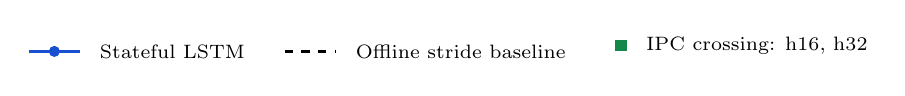
\begin{tikzpicture}[font=\scriptsize]
\draw[lstmblue,thick] (0,0)--(0.65,0); \fill[lstmblue] (0.325,0) circle (2pt);
\node[anchor=west] at (0.78,0) {Stateful LSTM};
\draw[black,dashed,thick] (3.25,0)--(3.90,0);
\node[anchor=west] at (4.03,0) {Offline stride baseline};
\fill[crossgreen] (7.45,0) rectangle +(0.15,0.15);
\node[anchor=west] at (7.72,0.075) {IPC crossing: h16, h32};
\end{tikzpicture}
\end{center}

\begin{center}
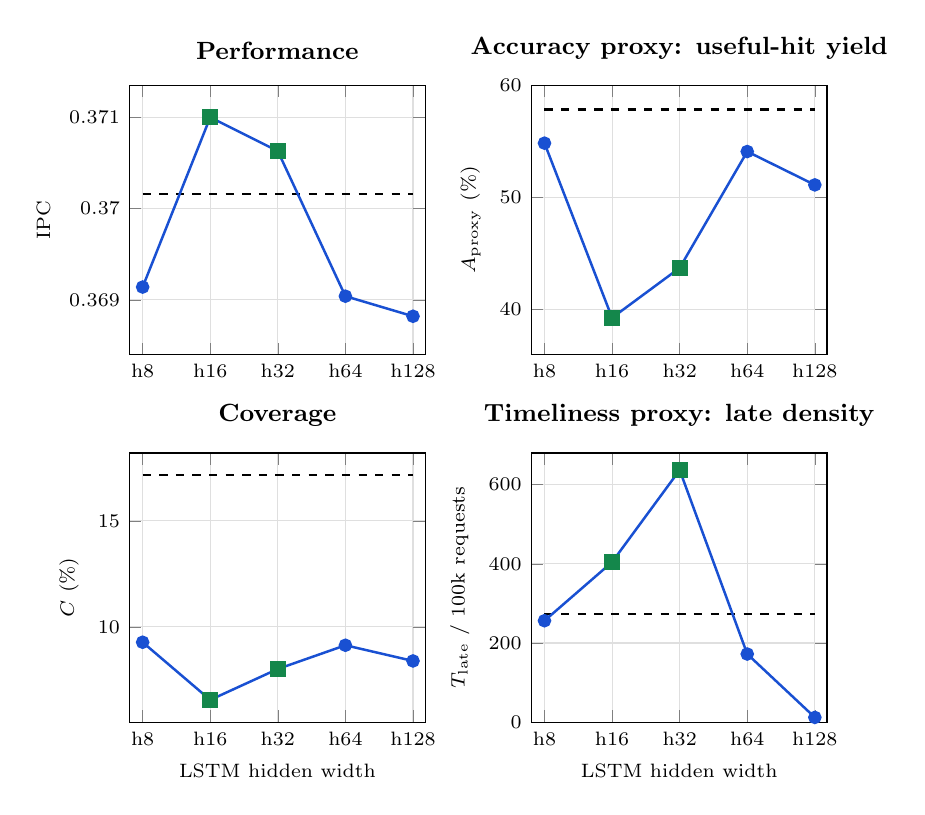
\begin{tikzpicture}
\begin{groupplot}[
 group style={group size=2 by 2,horizontal sep=1.35cm,vertical sep=1.25cm},
 width=0.44\textwidth,height=5.0cm,
 xmode=log,log basis x=2,xmin=7,xmax=145,
 xtick={8,16,32,64,128},xticklabels={h8,h16,h32,h64,h128},
 grid=major,grid style={gray!25},tick label style={font=\scriptsize},
 label style={font=\scriptsize},title style={font=\small\bfseries},
 every axis plot/.append style={line width=0.9pt},
]
\nextgroupplot[title={Performance},ylabel={IPC},ymin=0.3684,ymax=0.37135,
 yticklabel style={font=\scriptsize,/pgf/number format/fixed,/pgf/number format/precision=5}]
\addplot[black,dashed,domain=8:128,samples=2] {0.37016};
\addplot[lstmblue,mark=*] coordinates {(8,0.36914) (16,0.37100) (32,0.37063) (64,0.36904) (128,0.36882)};
\addplot[crossgreen,only marks,mark=square*,mark size=2.4pt] coordinates {(16,0.37100) (32,0.37063)};

\nextgroupplot[title={Accuracy proxy: useful-hit yield},ylabel={$A_{\rm proxy}$ (\%)},ymin=36,ymax=60]
\addplot[black,dashed,domain=8:128,samples=2] {57.8375};
\addplot[lstmblue,mark=*] coordinates {(8,54.8507) (16,39.2779) (32,43.7287) (64,54.1036) (128,51.1297)};
\addplot[crossgreen,only marks,mark=square*,mark size=2.4pt] coordinates {(16,39.2779) (32,43.7287)};

\nextgroupplot[title={Coverage},xlabel={LSTM hidden width},ylabel={$C$ (\%)},ymin=5.5,ymax=18.2]
\addplot[black,dashed,domain=8:128,samples=2] {17.1564};
\addplot[lstmblue,mark=*] coordinates {(8,9.2714) (16,6.5500) (32,8.0101) (64,9.1291) (128,8.3887)};
\addplot[crossgreen,only marks,mark=square*,mark size=2.4pt] coordinates {(16,6.5500) (32,8.0101)};

\nextgroupplot[title={Timeliness proxy: late density},xlabel={LSTM hidden width},ylabel={$T_{\rm late}$ / 100k requests},ymin=0,ymax=680]
\addplot[black,dashed,domain=8:128,samples=2] {273.8362};
\addplot[lstmblue,mark=*] coordinates {(8,256.2982) (16,404.4400) (32,636.9427) (64,172.1371) (128,12.0023)};
\addplot[crossgreen,only marks,mark=square*,mark size=2.4pt] coordinates {(16,404.4400) (32,636.9427)};
\end{groupplot}
\end{tikzpicture}
\end{center}

\vspace{-3pt}
\begin{center}\scriptsize
All legends and crossing indicators are outside the axes. Dashed lines are the offline stride primary comparator.
\end{center}

\newpage
\section*{Data $\rightarrow$ insight map}
\begin{center}\scriptsize
\begin{tabularx}{\textwidth}{@{}p{0.23\textwidth}p{0.35\textwidth}X@{}}
\toprule
Question & Direct evidence & Supported insight \\
\midrule
Why does h16 beat stride? & IPC rises 0.00084 while requests fall 43.8\%. However, useful hits fall 61.8\%, coverage falls 10.61 points, $A_{\rm proxy}$ falls 18.56 points, and late density rises. & The crossing is \textbf{not explained by higher measured accuracy, coverage, or timeliness}. Fewer requests may reduce bandwidth/pollution, or the remaining misses may differ in criticality, but those mechanisms are not yet counted.\\
Is h16 a saturation point? & h16 and h32 cross; h64 and h128 do not. Parameter count grows from 1,729 to 85,505 without monotonic IPC gain. & h16 is the first measured crossing, not a capacity saturation law. Width alone does not control outcome.\\
Does h128 look timely? & Late density is only 12.0, but IPC is 0.36882 and coverage is 8.39\%. & A very low late proxy can coexist with poor performance when the gate suppresses opportunities. It cannot be read alone.\\
Did stateful TBPTT matter? & Corrected h16 rises from the pre-fix 0.37090 to 0.37100; h32 rises from 0.37033 to 0.37063. & Correct recurrence slightly strengthens the measured crossing, but the qualitative non-monotonic result remains.\\
\bottomrule
\end{tabularx}
\end{center}

\section*{Evidence boundary and next counters}
\begin{center}\scriptsize
\begin{tabularx}{\textwidth}{@{}lXX@{}}
\toprule
Claim type & Supported now & Still required \\
\midrule
Performance & Matched replay establishes h16/h32 IPC crossings on this trace/window. & Multiple traces, seeds, and a fresh held-out window before selecting a final capacity.\\
Strict accuracy & $U/R$ gives request-event yield. & Accepted/filled unique prefetches, duplicate rejection, unused eviction, and pollution.\\
True timeliness & Late merges give one late-failure count. & Issue/fill/demand cycles and lead-time histograms.\\
Why IPC rises with more misses & The counters rule out ``more coverage'' and ``lower late density'' as explanations for h16/h32. & Bandwidth/MSHR occupancy, eviction/pollution, useful-prefetch lead time, and critical-miss stall cycles.\\
\bottomrule
\end{tabularx}
\end{center}

\section*{Reproducibility anchors}
\begin{itemize}\scriptsize
\item Run: \texttt{602\_offline\_lstm\_stride\_stateful\_v2\_seed7}; analyzer status \textbf{PASS}.
\item Train content SHA256: \texttt{2564c753145acde5a2c7a9f94904366e18aa7ebdd0a10003d2944104c854a594}.
\item Evaluation content SHA256: \texttt{36ce707c2f27023e400f16c2cc2054c61e20b54d5dc26959c6857ef8e8e87d2f}.
\item Offline stride list SHA256: \texttt{f2440cefff0d476ce12ec715c232579a15ad0e6e6a94767aea6f9e7dd8fd9d9f}.
\end{itemize}

\end{document}
